\documentclass[aspectratio=169]{beamer}

\usepackage[utf8]{inputenc}
\usepackage[english]{babel}
\usepackage{multicol}
\usepackage{tabulary}
\usepackage{hyperref}
\usepackage{tikz}
\usetikzlibrary{shapes, arrows, trees, calc}
\usepackage{mathtools}

\let\oldsection\section
\renewcommand{\section}[1]{
    \oldsection{#1}	
    \subsection{}
}

\setbeamerfont{section in toc}{size=\LARGE}

\newenvironment{myframe}[1][t]{\begin{frame}[#1]{\secname}{\subsecname}}{\end{frame}}

\usetheme{cranfielduniversity}

\usepackage[sorting=none, backend=biber, style=numeric, doi=false, isbn=false, url=false, eprint=false, date=year, hyperref]{biblatex}

\addbibresource{../library.bib}
\addbibresource{../my_references.bib}

\author{Baptiste NOGARET}
\title{Automated food log}
\date{21\textsuperscript{st} July 2016}

\supervisor{Dr Stefan RÜGER}

\setcounter{tocdepth}{1}

\begin{document}
	
	\begin{frame}[plain]
		\titlepage
	\end{frame}
    
    \begin{frame}{Table of contents}
        {
            \renewcommand{\baselinestretch}{1.5}\normalsize
            \begin{multicols}{2}
                \tableofcontents
            \end{multicols}
        }
    \end{frame}
    
    \section{Why a food log analysis system?}
    
    {
        % Disable footline for this frame
        \setbeamertemplate{footline}{}
    	\begin{myframe}
            \vspace{-0.4cm}
            \begin{figure}[h]
                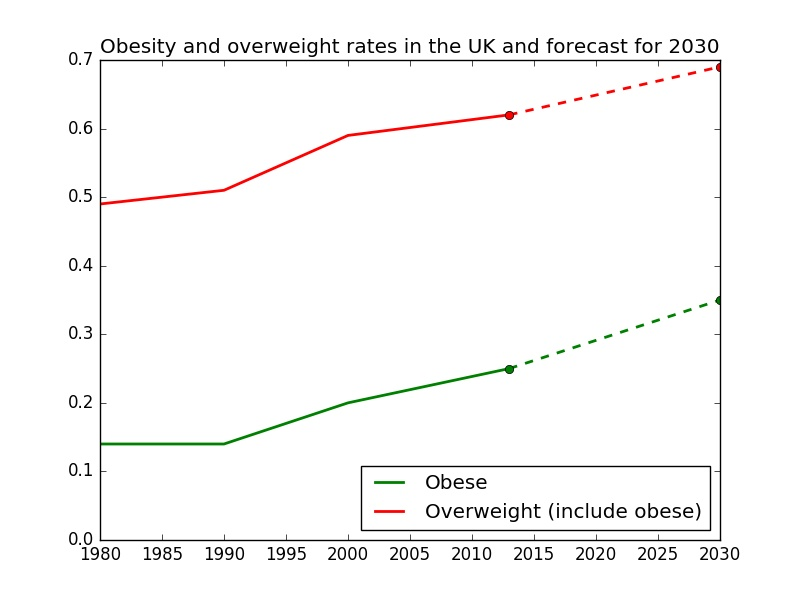
\includegraphics[width=0.5\textwidth,  height=0.45\textwidth ]{../img/obesity_uk}
                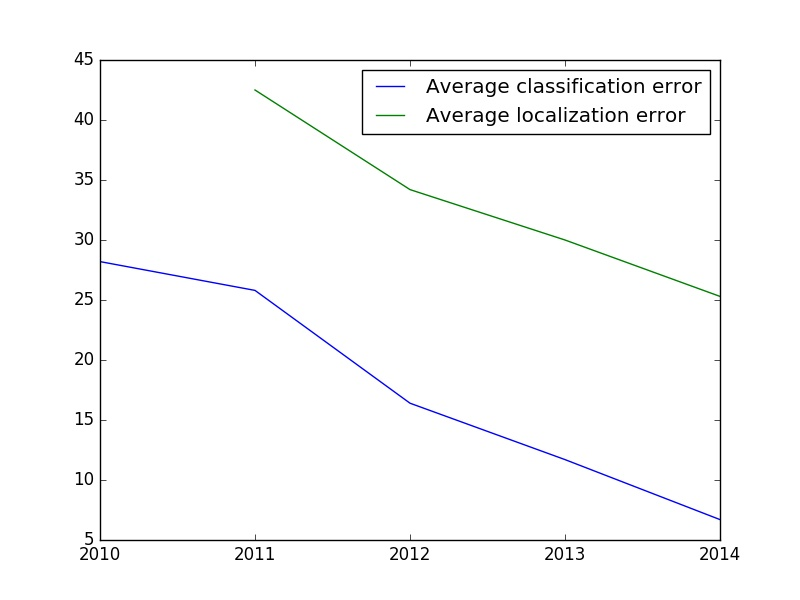
\includegraphics[width=0.5\textwidth,  height=0.455\textwidth ]{../img/imagenet}
            \end{figure}
    	\end{myframe}
    }
    
     \section{Overall process}
     
     \begin{myframe}[c]
         Roughly copying the procedure of FoodLog \cite{Kitamura2009, Kitamura2008, DeSilva2011, Aizawa2013, Kagaya2014}:
         \begin{itemize}
             \item Generate a relevant dataset
             \item Extract characteristic
             \item Learn
             \item For a new picture from a user, classify and estimate intake
         \end{itemize}
         Focus on the first three points
     \end{myframe}
    
    \section{Challenges}
    {
        \author{}
        \begin{myframe}
            \vspace{-0.3cm}
            \begin{columns}
                \column{0.5\textwidth}
                \centering
                High intra-class variability
                \begin{figure}[h]
                    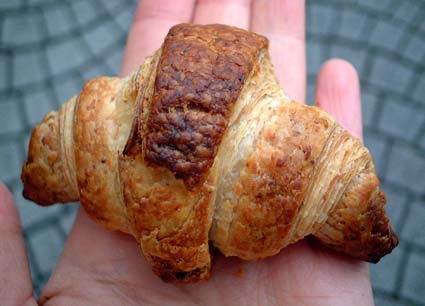
\includegraphics[width=0.7\textwidth, height=0.4\textwidth]{../img/croissant_2}
                    \vfill
                    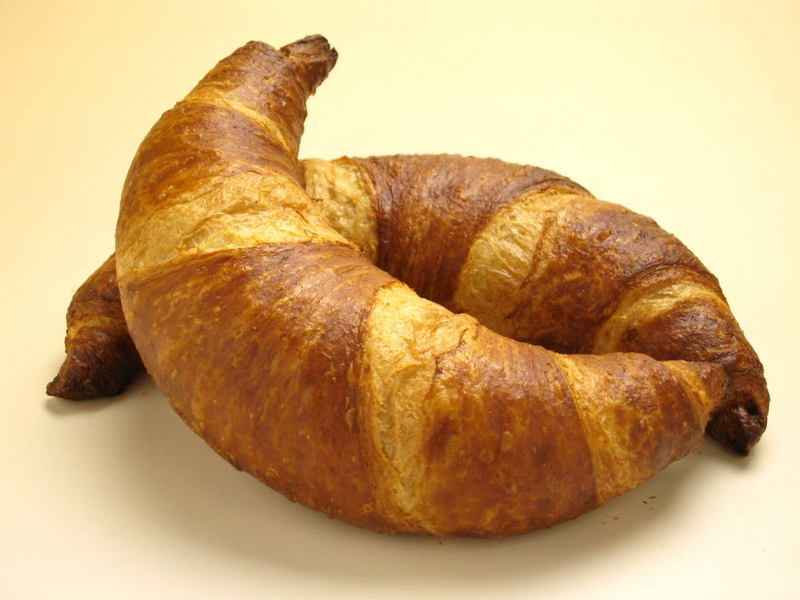
\includegraphics[width=0.7\textwidth, height=0.4\textwidth]{../img/croissant_3}
                \end{figure}
                
                \column{0.5\textwidth}
                \centering
                Low inter-class variability
                
                \begin{figure}[h]
                    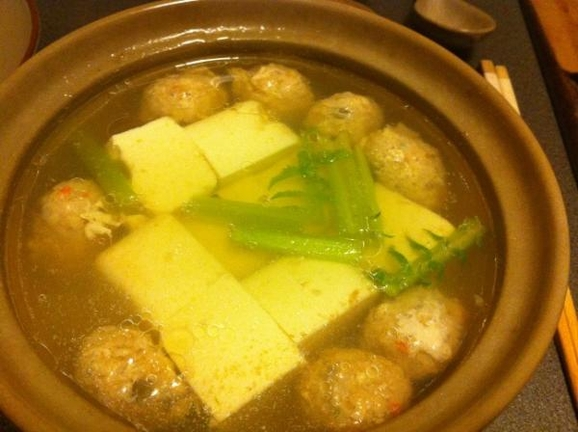
\includegraphics[width=0.7\textwidth, height=0.4\textwidth]{../img/clear_soup}
                    \vfill
                    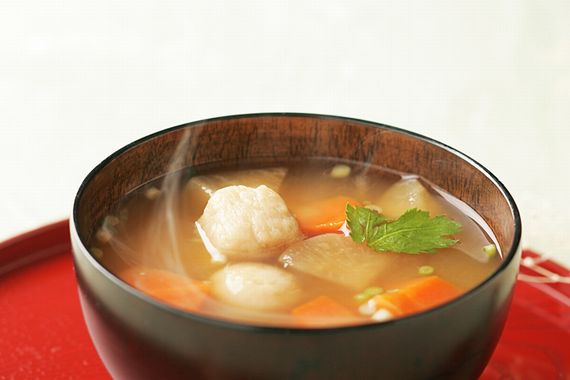
\includegraphics[width=0.7\textwidth, height=0.4\textwidth]{../img/miso_soup}
                \end{figure}
            \end{columns}
        \end{myframe}
    }

    \section{Dataset}
    
     \begin{myframe}
         \begin{center}
             %\setlength{\tabcolsep}{5pt} % Default value: 6pt
             \renewcommand{\arraystretch}{1.3} % Default value: 1
             \begin{tabulary}{\textwidth}{|| c | C C C C C||}
                 \hline
                 Name & Release date & Number of pictures & Type of food & Number of classes & Multiple food items \\
                 \hline\hline
                 PFID \cite{Chen2009} & 2009 & 4545 & American fast-food  & 101 & No \\
                 \hline
                 UEC FOOD 100 \cite{Matsuda2012a} & 2012 & 14361 & Japanese & 100  & Yes \\
                 \hline
                 FIDS 30 \cite{FIDS30} & 2013 & 971 & Fruit & 30 & No \\
                 \hline
                 ETHZ Food-101 \cite{Bossard2014} & 2014 & 101 000 & European & 100 & No \\
                 \hline
                 FooDD \cite{ParisaPouladzadehAbdulsalamYassine2015} & 2015 & 3000 & Fruit & 23 & Yes \\
                 \hline
                 \textbf{UEC FOOD 256} \cite{Kawano2015} & \textbf{2015} & \textbf{31395} & \textbf{World} & \textbf{256}  & \textbf{Yes} \\ 
                 \hline
             \end{tabulary}
        \end{center}
    \end{myframe}
    
    {
        \author{}
        \subsection{Example of multi-items}
        
        \begin{myframe}
            \begin{figure}[h]
                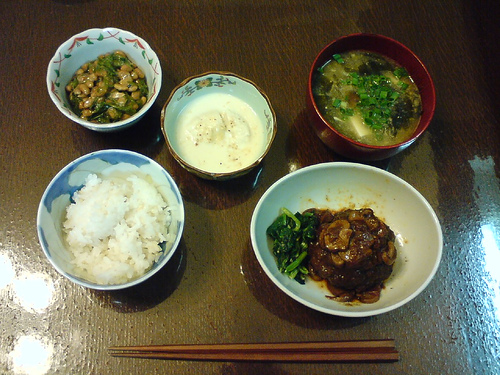
\includegraphics[width=0.4\textwidth,  height=0.4\textwidth ]{../img/multiple_food_items_1}
                \vspace{2cm}
                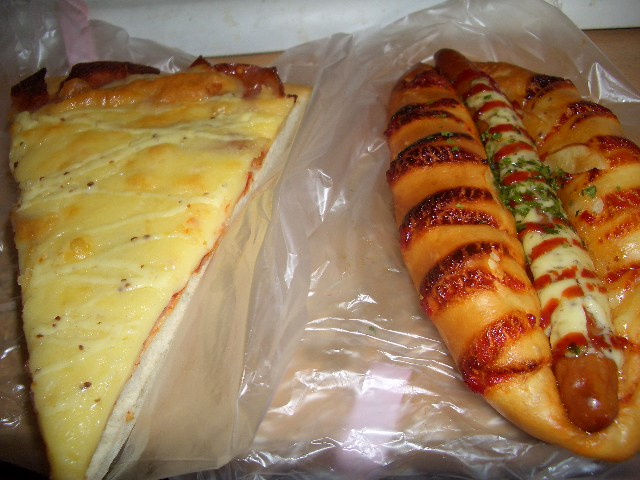
\includegraphics[width=0.4\textwidth,  height=0.4\textwidth ]{../img/multiple_food_items_4}
            \end{figure}
        \end{myframe}
    }
    
    \section{Feature description}
    
    \subsection{Bag of visual words}
    
    \begin{myframe}
        Common feature descriptor, use in \cite{Chen2009, Hoashi2010a, Bettadapura2015}
        \vspace{0.5cm}
        \begin{center}
            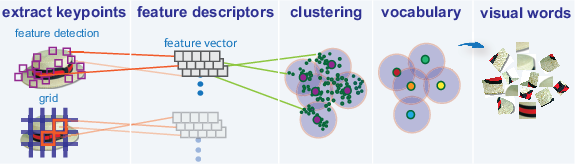
\includegraphics[scale=0.9]{../img/bow.png}
        \end{center}
    \end{myframe}
    
    \subsection{Local binary pattern}
    
    \begin{myframe}
        Use in \cite{Zong2010, Nguyen2014} for texture classification
        
        \begin{center}
            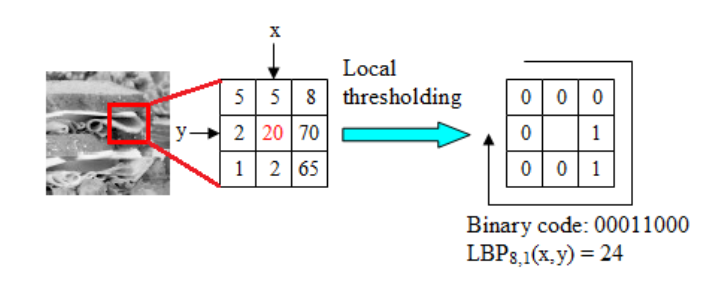
\includegraphics[scale=0.55]{../img/lbp}
        \end{center}
    \end{myframe}
    
    \subsection{Color moments and histograms}
    
    \begin{myframe}
        \vspace{-0.5cm}
        \begin{columns}
            \column{0.6\textwidth}
            \centering
            % Joint histogram:
            \begin{figure}[h]
                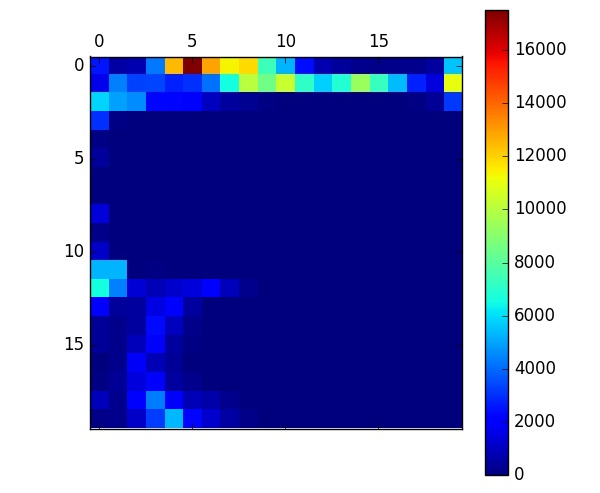
\includegraphics[scale=0.35]{../img/joint_histogram}
            \end{figure}
            
            \column{0.4\textwidth}
            \centering
            Mean:
            $$ \mu = \frac{1}{n} \sum_{i = 1}^{n} x_i $$
            Variance:
            $$ \operatorname {Var} (X)=\sum _{i=1}^{n}p_{i}\cdot (x_{i}-\mu )^{2} $$
        \end{columns}
    \end{myframe}
    
    \section{Classifiers}
    
    \subsection{Tree and random forest}
    
    \begin{myframe}
        \begin{center}
            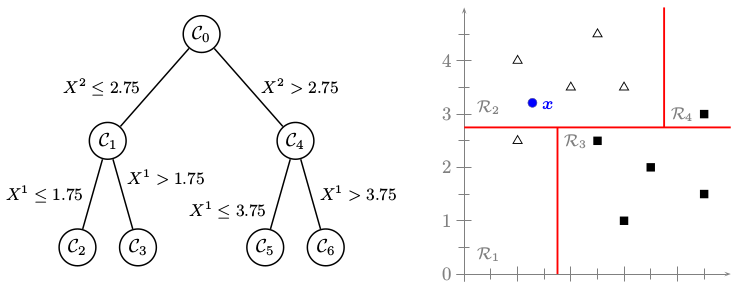
\includegraphics[scale=0.50]{../img/decision_tree_simple_example}
        \end{center}
    \end{myframe}
    
    \subsection{SVM}
    
    \begin{myframe}
        \vspace{-1cm}
        \begin{center}
            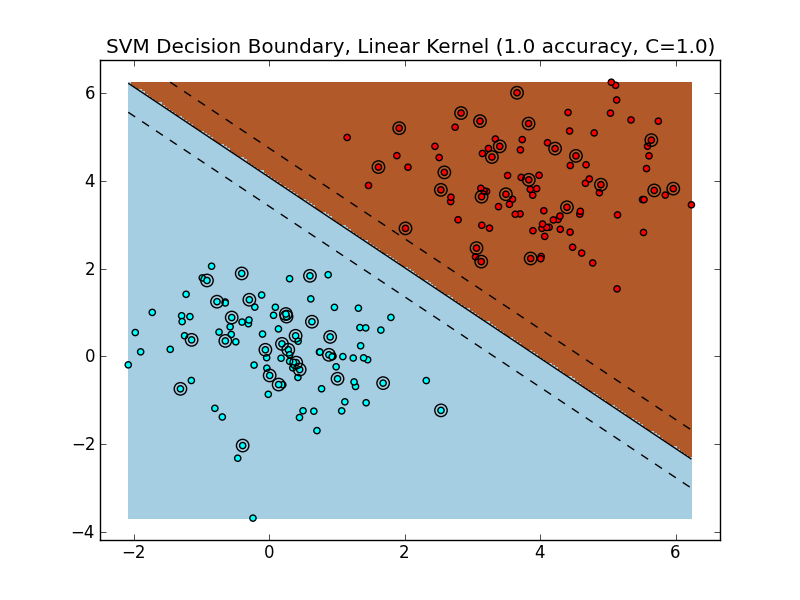
\includegraphics[scale=0.5]{../img/svm_linear}
        \end{center}
    \end{myframe}
    
    \subsection{SVM and kernel trick}
    
    \begin{myframe}
        %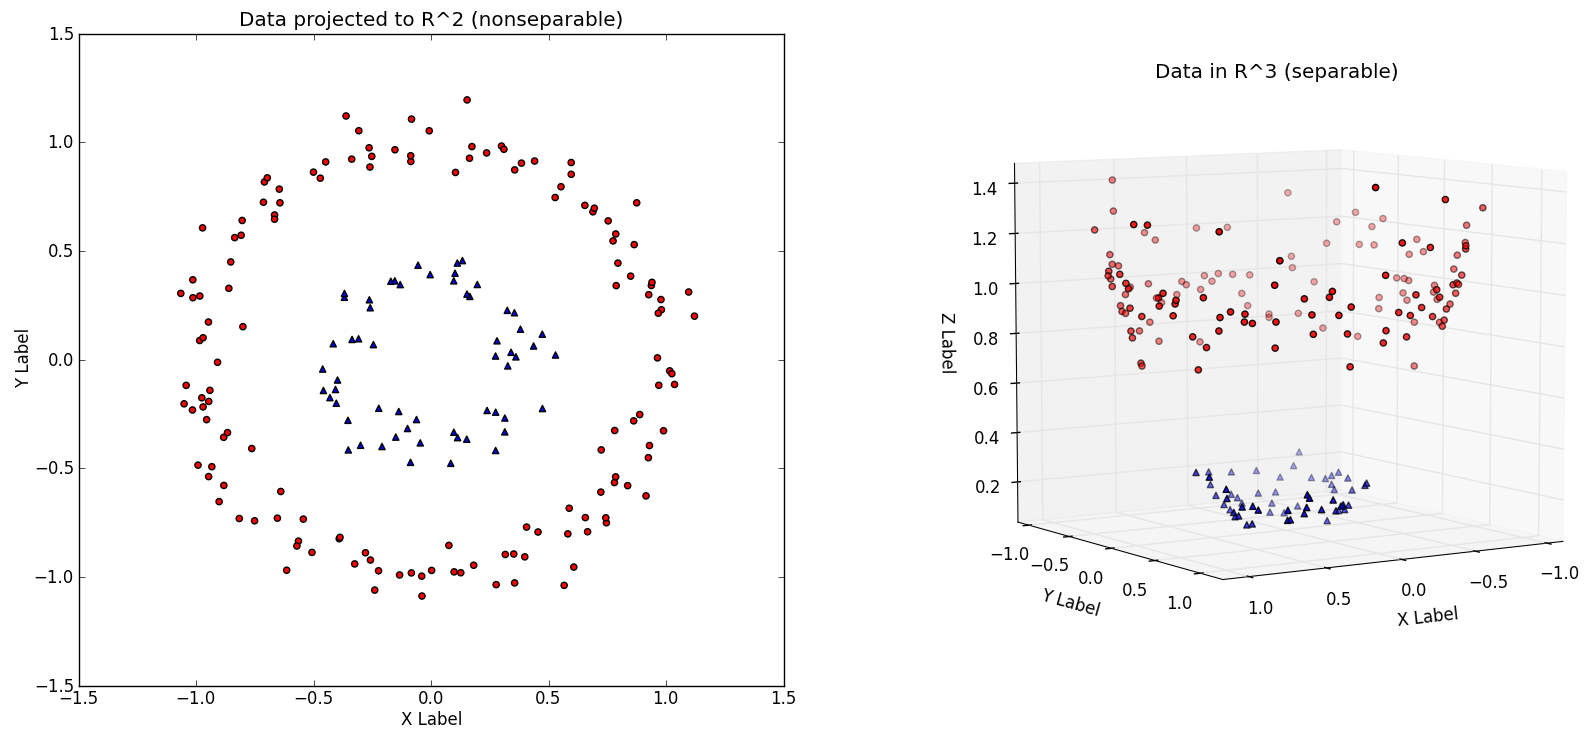
\includegraphics[scale=0.55]{../img/svm_data_2d_to_3d.png}
        \begin{center}
            \begin{tikzpicture}
                \node[anchor=south west,inner sep=0] (image) at (0,0) {
                    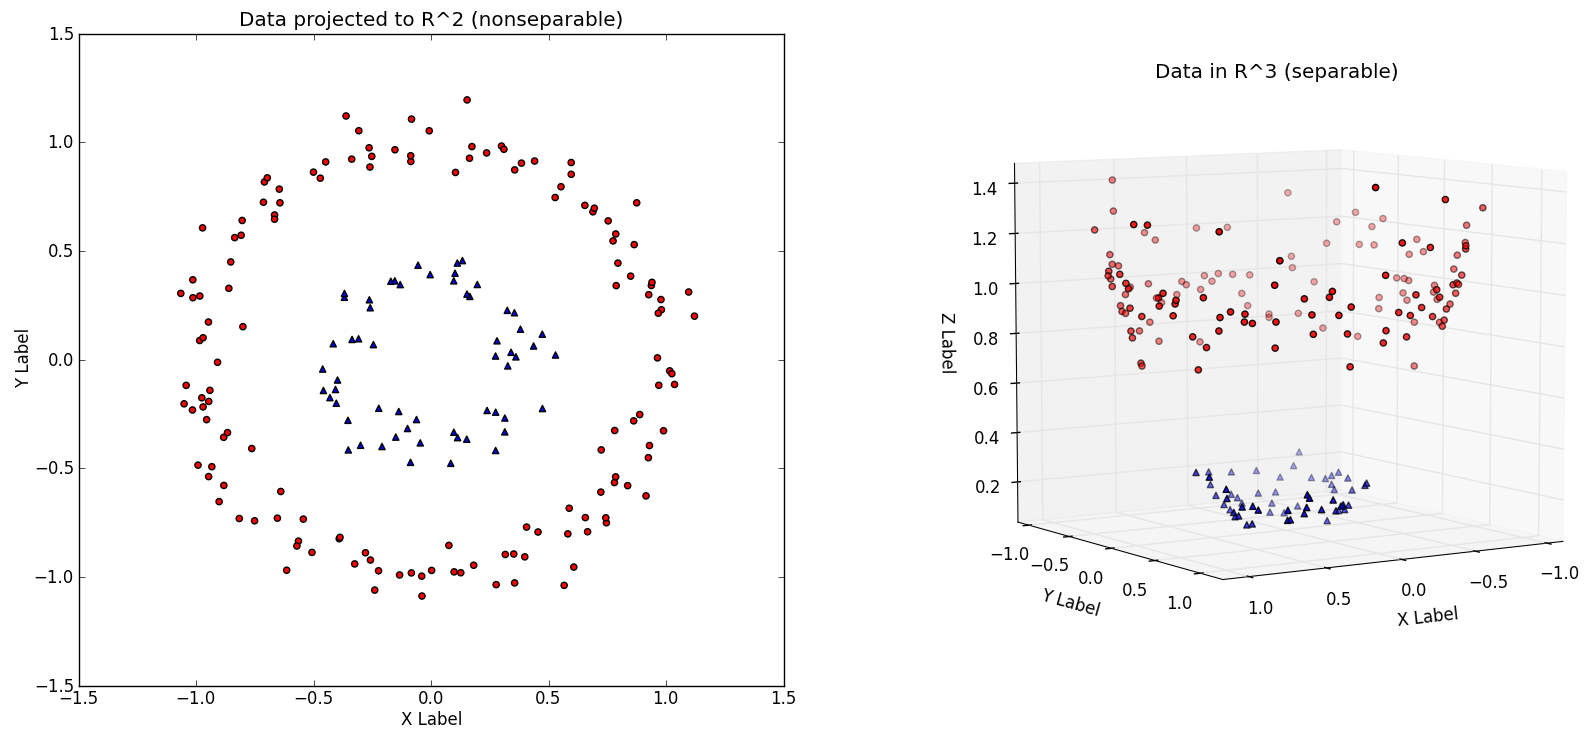
\includegraphics[scale=0.3]{../img/svm_data_2d_to_3d.png}
                };
            \end{tikzpicture}
        \end{center}        
    \end{myframe}
    
    \subsection{CNN}
    
    {
        \setbeamertemplate{footline}{}
        \setbeamertemplate{headline}{}
        \begin{myframe}
            \vspace{-0.35cm}
            \begin{center}
                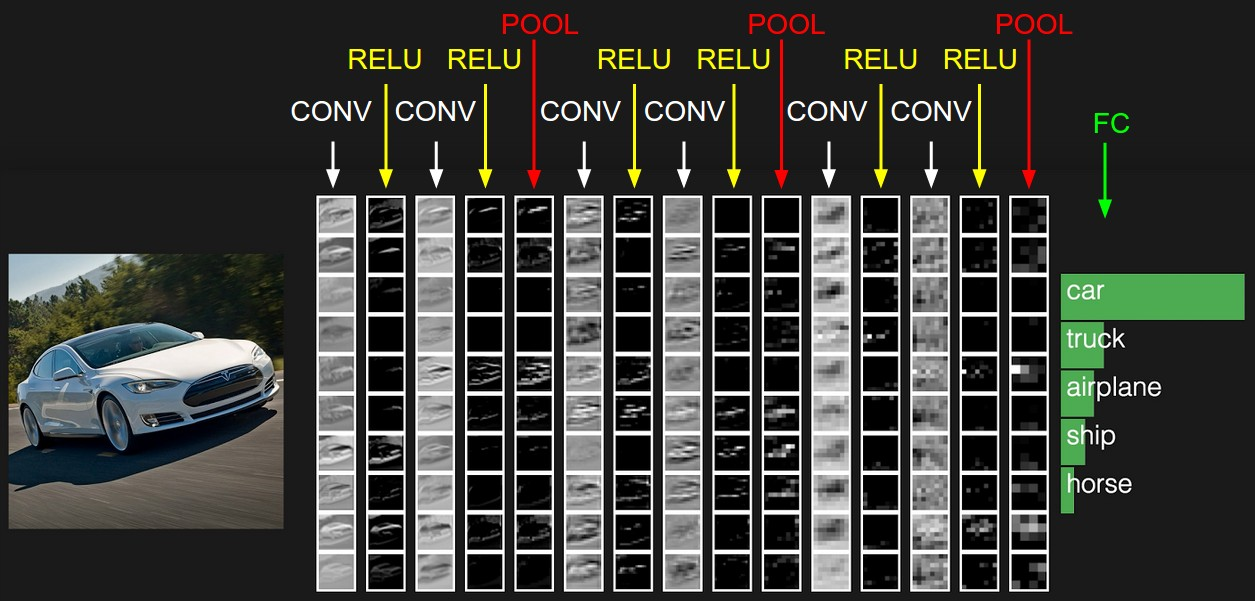
\includegraphics[scale=0.3]{../img/cnn_simple_example.jpeg}
            \end{center}
        \end{myframe}
    }
    
    \section{Structure}
    
    {
        \setbeamertemplate{footline}{}
        \begin{myframe}
            \vspace{-0.5cm}
            \centering
            \tikzstyle{block} = [rectangle, draw, text width=3cm, text centered, rounded corners,  fill=blue!20]
            \tikzstyle{line} = [draw,thick, -latex']
            \tikzstyle{cloud} = [draw, ellipse, text width=3cm, text centered]
            \tikzstyle{edge from parent}=[->,thick,draw]
            
            \begin{tikzpicture}[auto,edge from parent fork down]
            \tikzstyle{level 1}=[sibling distance=75mm,level distance=10ex]
            %\tikzstyle{level 2}=[sibling distance=50mm,level distance=10ex]
            %\tikzstyle{level 3}=[sibling distance=50mm,level distance=10ex]
            % Place nodes
            \node [cloud, fill=red!10] (cst) {Dataset}
            child{node [cloud, fill=green!10] (pmt) {Validation set}
                child{node [block, fill=blue!10] (opm) {Hyper-parameter optimization}}
            }
            child{node [cloud, fill=green!10] (ra) {Train / test sets}
                child{node [block, fill=blue!10] (cr) {Segmentation}}
            };
            \node[below of= cr, block, fill=blue!10](sse){Feature description};
            \node[below of= sse, block, fill=blue!10](ow){Classification};
            \node[below of= ow, block, fill=red!10](isse){Result};
            %% Draw edges
            \path [line] (cr.south) -- (sse.north);
            \path [line] (opm.east) -- (cr.west);
            \path [line] (opm.south) -- (ow.west);
            \path [line] (sse.south)--(ow.north);
            \path [line] (ow.south) -- (isse.north);
            \end{tikzpicture}
        \end{myframe}
    }
    
    \section{Results}
    
    \subsection{Segmentation}
    
    \begin{myframe}
        \begin{columns}
            \column{0.5\textwidth}
            Using a DCNN pre-trained on \cite{zhang2015SOD} to detect saliency object
            
            \vspace{0.5cm}
            
            Correcteness metric: As describe in \cite{pascalVoc2012}, must have an intersection over union greater than 50 \%
            $$IoU = \frac{area(B_p \cap B_{gt})}{area(B_p \cup B_{gt})}$$
            
            \column{0.5\textwidth}
            \begin{center}
                \renewcommand{\arraystretch}{1.3} % Default value: 1
                \begin{tabular}{||c | c c||} 
                    \hline
                    Metric & My method & DCNN from \cite{Bolanos2016} \\
                    \hline\hline
                    Accuracy & \textbf{73 \%} & 60 \% \\ 
                    \hline
                    Recall &  \textbf{74 \%} & 80 \% \\
                    \hline
                    Precision &  \textbf{79 \%} & 70 \% \\
                    \hline
                \end{tabular}
            \end{center}
        \end{columns}
    \end{myframe}
    
    \subsection{Classification}
    
    \begin{myframe}
          \begin{center}
              \renewcommand{\arraystretch}{1.3} % Default value: 1
              \begin{tabulary}{\textwidth}{|| c | C||}
                  \hline
                  Method & Average accuracy \\
                  \hline\hline
                  CNN as descriptor + RF & \textbf{40 \%} \\ 
                  \hline
                  BoW (1000 words)+ SVM with $\chi^2$ & 10 \% \\ % made up!
                  \hline
                  LBP + color historams and moments + Decision tree & 5 \% \\ 
                  \hline
                  LBP + color historams and moments + SVM & 11 \% \\ % made up!
                  \hline
                  LBP + color historams and moments + RF & 16 \% \\ % improved!
                  \hline
                  \hline
                  DCNN from \cite{Bolanos2016} & 63 \%\\
                  \hline 
                  DCNN from \cite{Yanai2015} & 67 \%\\
                  \hline 
                \end{tabulary}
            \end{center}
    \end{myframe}
    
    \subsection{Segmentation and classification}
    
    \begin{myframe}
        Segmentation: DCNN followed by the classification: CNN as a descriptor and RF
        
        \begin{columns}
            \column{0.5\textwidth}
            \begin{center}
                UEC FOOD 256
                \vspace{0.5cm}
                
                \renewcommand{\arraystretch}{1.3} % Default value: 1
                \begin{tabulary}{\textwidth}{|| c | C C||}
                    \hline
                    Accuracy & My method & DCNN from \cite{Bolanos2016} \\
                    \hline\hline
                    Overall & \textbf{28 \%} & 36 \% \\ 
                    \hline
                    Segmentation &  \textbf{74 \%} & 60 \% \\
                    \hline
                    Classification &  \textbf{38 \%} & 60 \% \\
                    \hline
                \end{tabulary}
            \end{center}
            
            \column{0.5\textwidth}
            \begin{center}
                UEC FOOD 100
                \vspace{0.5cm}
                
                \renewcommand{\arraystretch}{1.3} % Default value: 1
                \begin{tabulary}{\textwidth}{|| C | C c c||} 
                    \hline
                    Accuracy & My method & \cite{Shimoda2015} & \cite{Kawano2014} \\
                    \hline\hline
                    Overall & \textbf{33 \%} & - & - \\ 
                    \hline
                    Segmentation &  \textbf{67 \%} & 60 \% & - \\
                    \hline
                    Classification &  \textbf{50 \%} & -  & 72 \% \\
                    \hline
                \end{tabulary}
            \end{center}
        \end{columns}
    \end{myframe}
    
    \section{Future work and comment}
    
    \begin{myframe}
        \begin{columns}
            \column{0.5\textwidth}
            \renewcommand{\baselinestretch}{1.5}\normalsize
            \begin{itemize}
                \item Regroup the classification in 5 big categories for food intake as in \cite{Aizawa2013}
                
                \item Use a better feature descriptor / classifier
                
                \item Segmentation suppose that the food is the main focus of the picture
            \end{itemize}
            \column{0.5\textwidth}
            \centering
            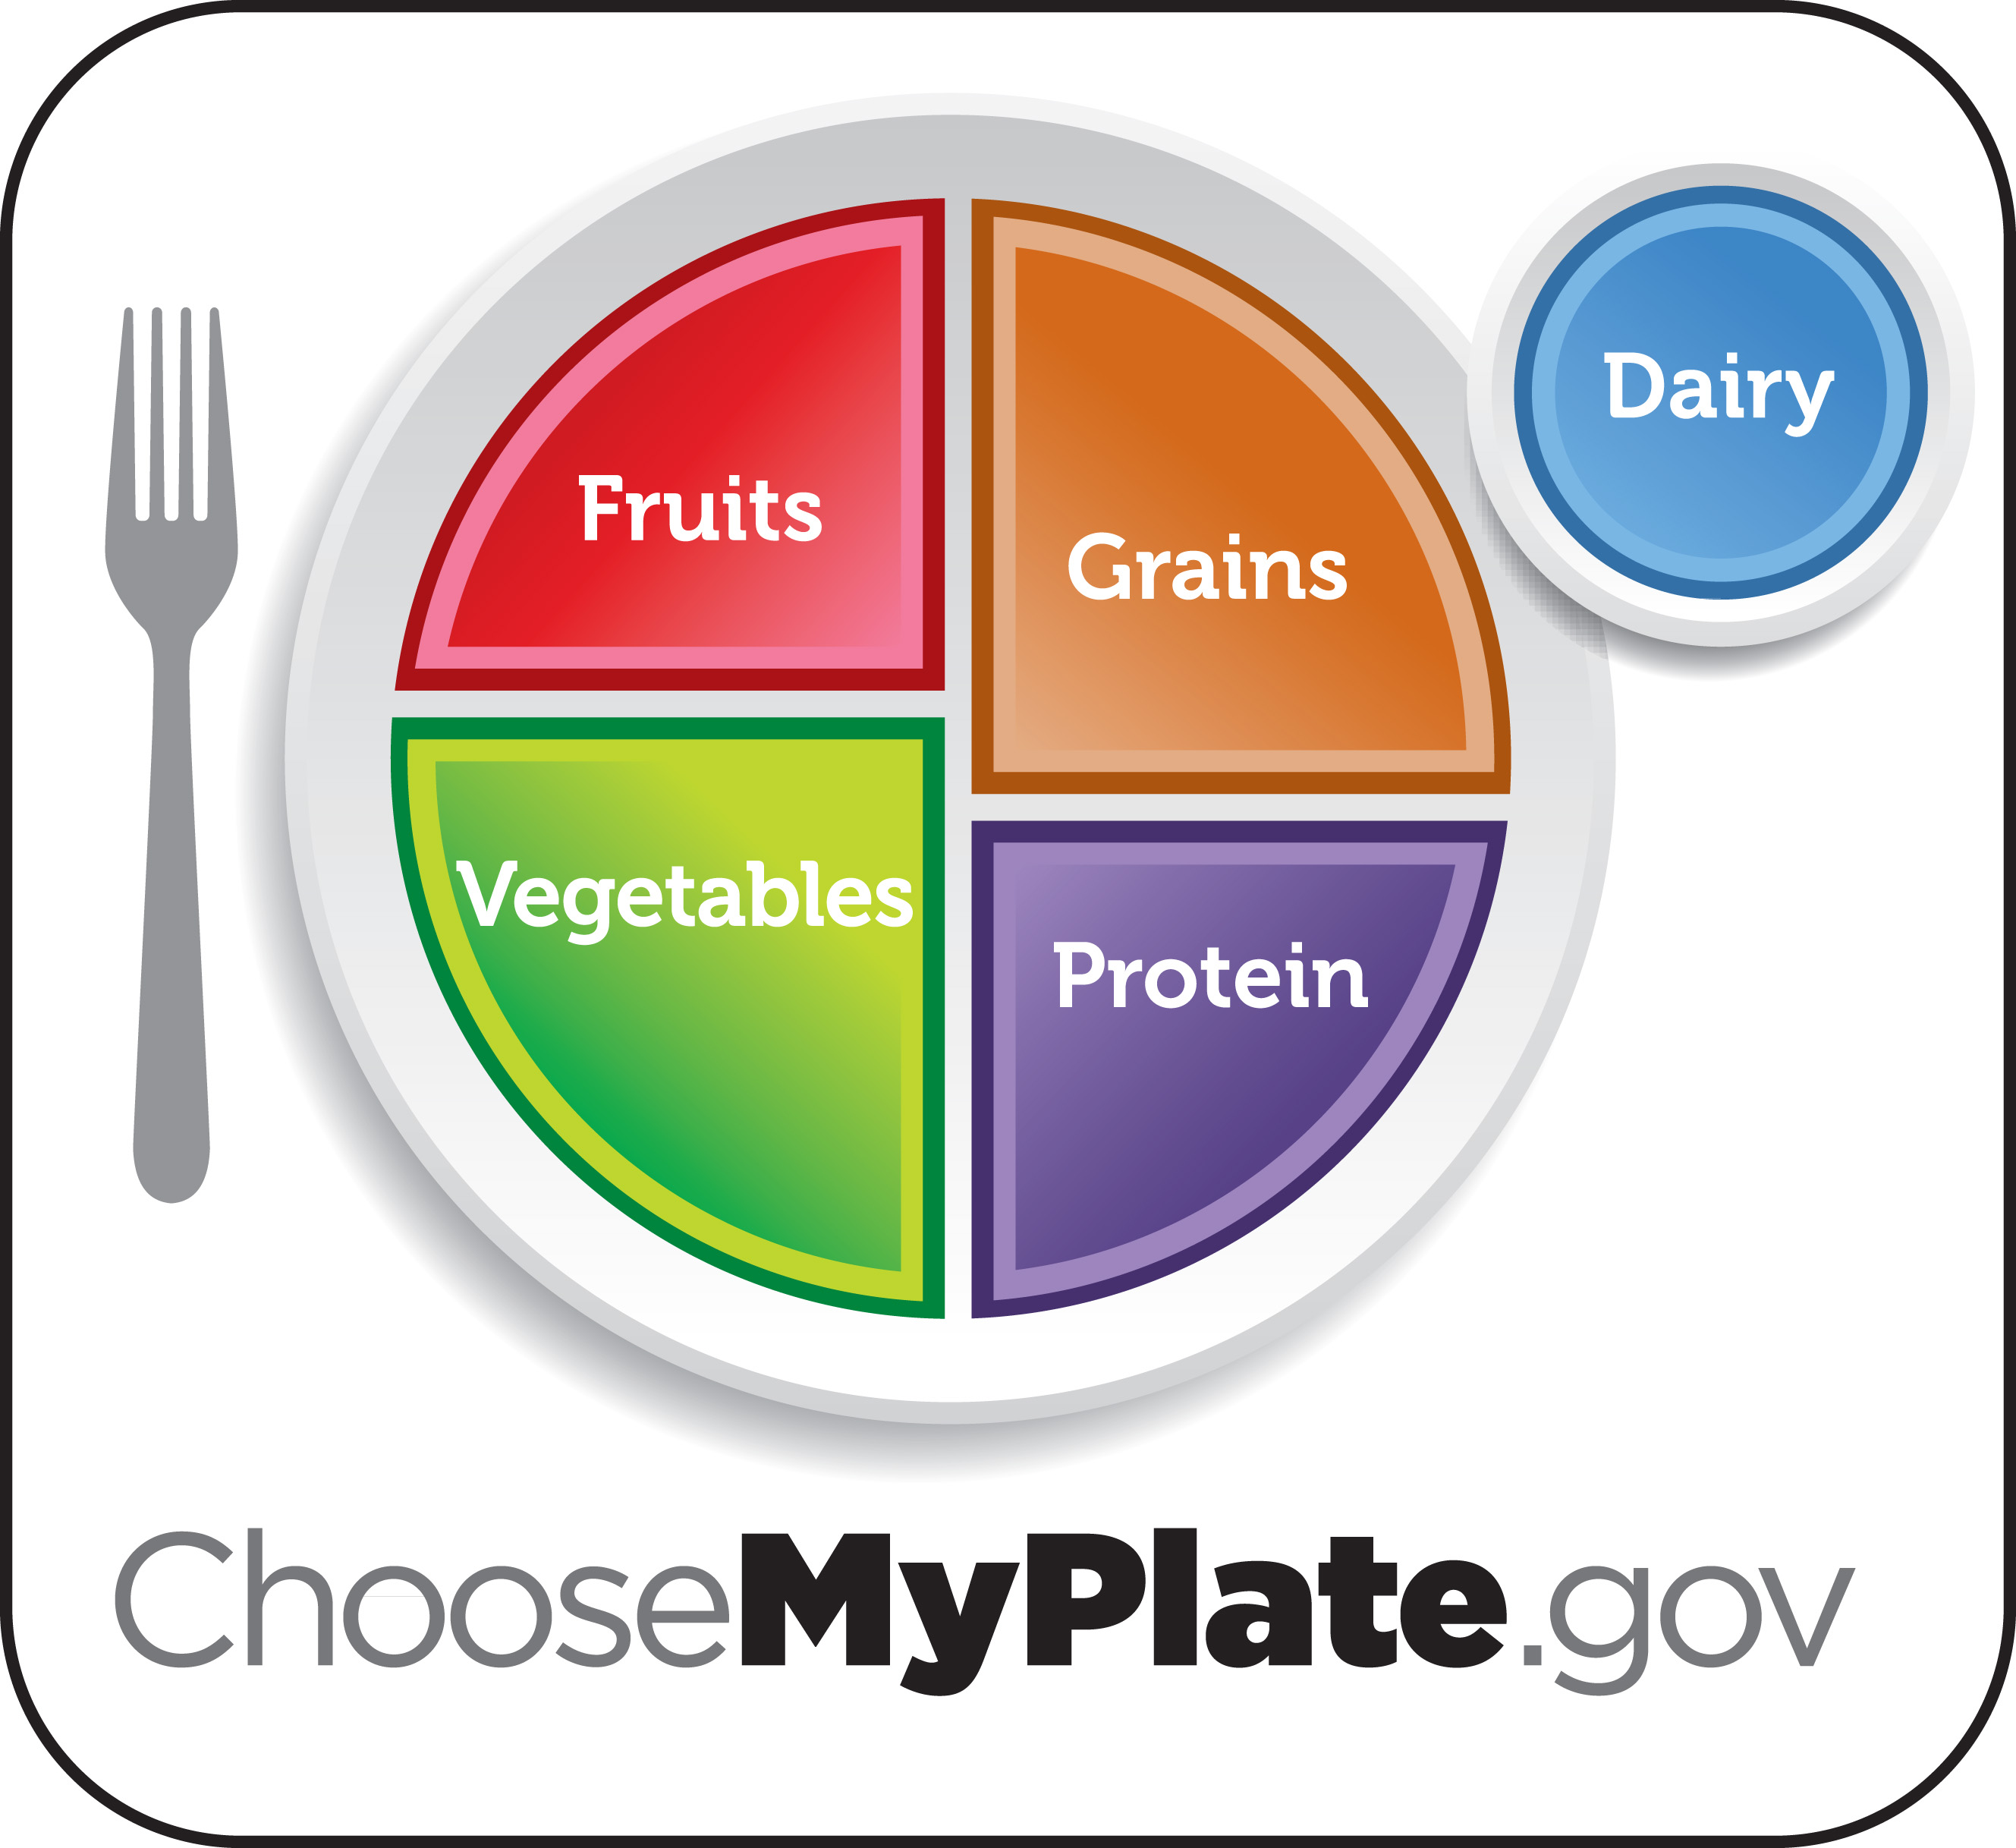
\includegraphics[scale=0.25]{../img/choosemyplate.jpg}
        \end{columns}
        
    \end{myframe}
    
     \section{Question}
    
    {
        % Disable footline for this frame
        % \setbeamertemplate{footline}{}
        \begin{frame}{Food log analysis - Baptiste NOGARET}{}
            \begin{columns}
                \column{0.5\textwidth}
                Segmentation and classfication applied on two reference datasets
                
                \vspace{0.5cm}
                
                Obtain better segmentation than the reference
                
                \vspace{0.5cm}
                
                Overall accuracy of 28 \% (to date, the best result is 36 \% in \cite{Bolanos2016}).
                
                \column{0.5\textwidth}
                \centering
                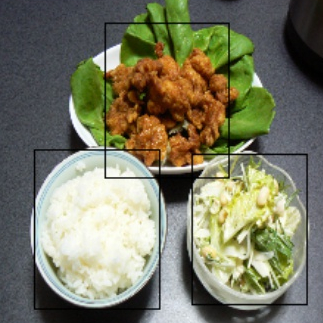
\includegraphics[scale=0.5]{../img/seg_97_gt}
            \end{columns}
        \end{frame}
    }
    
    \section{References}
    
    \begin{myframe}[t, allowframebreaks]
        \printbibliography[heading=none]
    \end{myframe}
   
\end{document}